% ------------------------------------------------------------------------------------------- %
%                                    Resultados e Discussão                                   %
% ------------------------------------------------------------------------------------------- %
\chapter{Resultados}\label{cap:resultados}

% ------------------------------------ Escopo do Sistema ------------------------------------ %
\section{Escopo do sistema}\label{sec:escopoSistema}

O sistema Contrate um Cientista terá como objetivo conectar organizações que possuem demandas específicas de pesquisa, desenvolvimento ou inovação com laboratórios científicos 
que possuem expertise para atender essas necessidades. Utilizando modelos de Inteligência Artificial, o sistema será capaz de analisar competências e demandas, garantindo um 
match eficiente e personalizado.

Abrange dois tipos de usuários: organizações e laboratórios científicos. Onde as organizações são responsáveis por criar as demandas e favoritar os cientistas 
pré selecionados pelos modelos de Inteligência Artificial. E os laboratórios científicos responsáveis em cadastrar todos os recursos que possuem.

Os modelos de Inteligência Artificial são utilizados para encontrar os laboratórios que são aptos para uma demanda específica, levando em consideração palavras-chave, 
equipamentos e softwares.

A organização poderá selecionar os laboratórios que possui maior interesse (dentre os laboratórios aptos) para que os usuários do tipo laboratórios científico possa 
visualizar as especificações daquela demanda.

% ----------------------------------- Modelagem do Sistema ---------------------------------- %
\section{Modelagem do sistema}\label{sec:modelagemSistema}

A maior dificuldade atualmente, se concentra nos responsáveis do departamento que faz esse match entre uma demanda e um cientista nas universidades.
Pensando nisso, o sistema deveria ser de fácil acesso à esses responsáveis, por isso, o App foi uma solução que melhor se enquadraria. 
Finalmente, foi realizado um diagrama para que seja facilmente entendido quais seriam organizados os projetos necessários, juntamente com suas tecnologias, conforme \autoref{fig:fluxograma-comunicacao}.

\begin{figure}[htpb]
    \captionsetup{width=0.43\textwidth}
    \caption{Diagrama da plataforma.}
    \label{fig:fluxograma-comunicacao}
    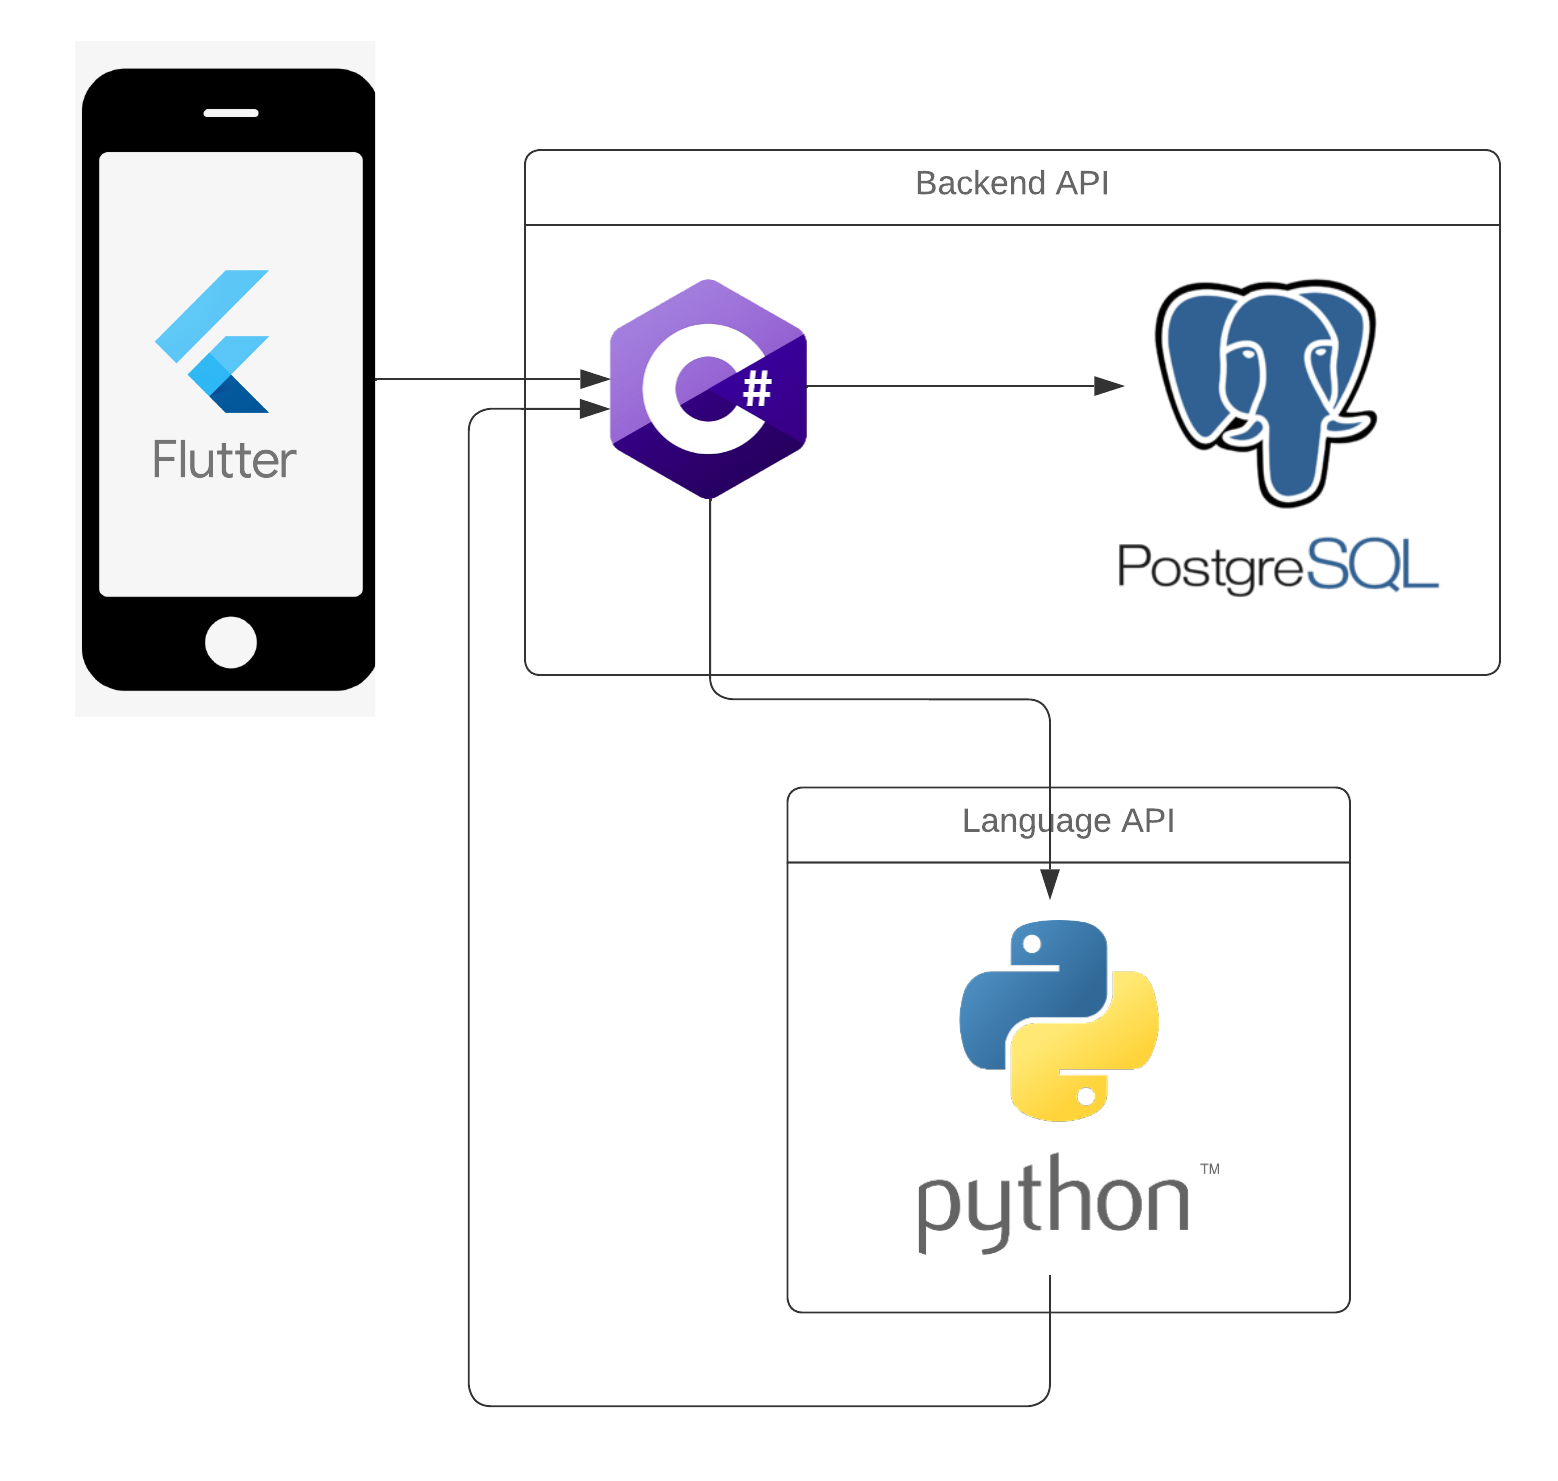
\includegraphics[scale=0.8]{fluxograma-comunicacao}
    \fonte{}
\end{figure}

Como a função principal, é a criação de demandas, foi possível entender melhor os passos através do diagrama \autoref{fig:diagrama-sequencia}.

\begin{figure}[htpb]
    \captionsetup{width=0.43\textwidth}
    \caption{Diagrama de sequência de criação de demanda.}
    \label{fig:diagrama-sequencia}
    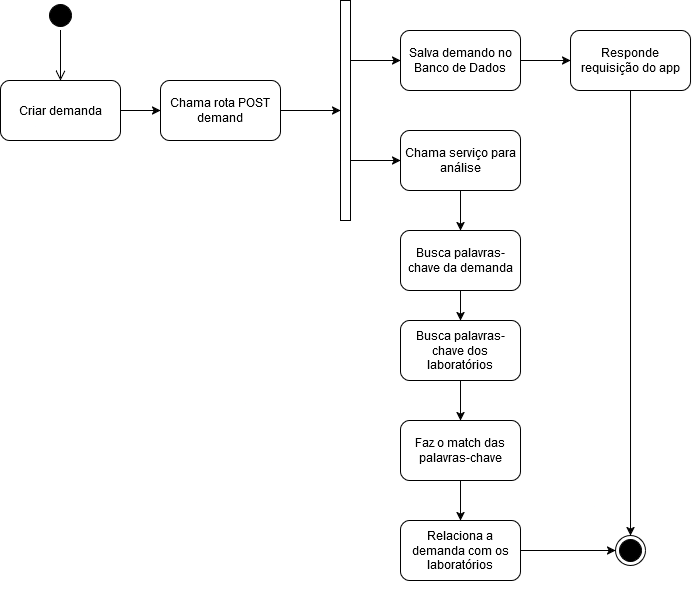
\includegraphics[scale=0.8]{diagrama-sequencia}
    \fonte{}
\end{figure}

\renewcommand{\labelenumii}{\arabic{enumi}.\arabic{enumii}}
\renewcommand{\labelenumiii}{\arabic{enumi}.\arabic{enumii}.\arabic{enumiii}}
\renewcommand{\labelenumiv}{\arabic{enumi}.\arabic{enumii}.\arabic{enumiii}.\arabic{enumiv}}

\subsection{Requisitos Funcionais}\label{subsec:ia1}
\begin{enumerate}
    \item O sistema deve disponibilizar um aplicativo
    \item O aplicativo deve ter uma página para o cadastro das organizações
	\begin{enumerate}
		\item Organização deve ter um email para login
		\item Organização deve ter uma senha
		\item Organização deve ter um nome
		\item Organização deve ter um cnpj
		\item Organização deve ter um email para contato
		\item Organização deve permitir uma descrição
	\end{enumerate}
    \item O aplicativo deve ter uma página para o cadastro de laboratórios
	\begin{enumerate}
		\item Laboratório deve ter um email para login
		\item Laboratório deve ter um código
		\item Laboratório deve ter uma data de fundação
		\item Laboratório deve ter palavras-chave
		\item Laboratório deve permitir uma descrição
		\item Laboratório deve permitir o cadastro dos seus certificados
		\item Laboratório deve ter um responsável
		\begin{enumerate}
			\item Responsável deve ter um nome
			\item Responsável deve permitir um departamento
			\item Responsável deve permitir um email
			\item Responsável deve permitir um telefone
		\end{enumerate}
		\item Laboratório deve ter um endereço
		\begin{enumerate}
			\item Endereço deve ter uma rua
			\item Endereço deve ter um número
			\item Endereço deve ter um bairro
			\item Endereço deve ter uma cidade
			\item Endereço deve ter um estado
			\item Endereço deve ter um país
			\item Responsável deve permitir um complemento
		\end{enumerate}
		\item Laboratório deve permitir uma descrição
		\item Laboratório deve permitir uma ou mais redes sociais
		\begin{enumerate}
			\item Rede social deve ter um tipo
			\item Rede social deve ter um link
		\end{enumerate}
		\item Laboratório deve permitir um ou mais equipamentos
		\begin{enumerate}
			\item Equipamento deve ter um nome
			\item Equipamento deve permitir uma descrição
			\item Equipamento deve permitir uma área
		\end{enumerate}
		\item Laboratório deve permitir um ou mais softwares
		\begin{enumerate}
			\item Software deve ter um nome
			\item Software deve permitir uma descrição
			\item Software deve permitir uma área
		\end{enumerate}
	\end{enumerate}
    \item O aplicativo deve ter uma página de login para os usuários
    \item O aplicativo deve permitir que o usuário faça o logout da sua conta
    \item O sistema deve permitir que um usuário visualize e edite as informações do seu perfil no sistema
    \item O aplicativo deve permitir que uma organização crie uma demanda
	\begin{enumerate}
		\item Demanda deve ter um título
		\item Demanda deve ter um departamento
		\item Demanda deve ter benefícios
		\item Demanda deve ter detalhes
		\item Demanda deve ter palavras-chave
		\item Demanda deve permitir uma descrição
		\item Demanda deve permitir restrições
	\end{enumerate}
	\item O sistema deve permitir que uma organização visualize todas suas demandas no sistema
	\item O sistema deve permitir que uma organização favorite laboratórios aptos para uma demanda específica
	\item O sistema deve permitir que uma organização visualize os laboratórios favoritados para cada demanda
	\item O sistema deve permitir que um laboratório visualize as informações da demanda após aquela organização o marcar como favorito
\end{enumerate}

\subsection{Requisitos Não-Funcionais}\label{subsec:ia1}
\begin{enumerate}
\item O sistema deve permitir ser instalado em sistema operacionais Android e iOs
\item O sistema deve ser usado a framework Dart
\item O sistema deve ser servido em C\#
\item O site deverá armazenar dados persistentes com PostgreSQL.
\item O sistema deve armazenar a senha criptografada
\item O sistema deve manter todas as informações protegidas de acordo com permissões do usuário logado
\item O sistema deve mostrar a organização os melhores candidatos para trabalhar naquela demanda
\item O sistema não deve travar até a análise de todos os laboratórios para aquela nova demanda
\end{enumerate}

O diagrama de caso de uso, para fácil visualização dos atores e suas respectivas ações {{diagrama-caso-de-uso}}

O banco de dados foi planejado para comportar os dois tipo de usuários diferentes (laboratório e organização), e para armazenar todos os dados relevantes para análise das demandas, de acordo com o diagrama da \autoref{fig:ERD}.

\begin{figure}[htpb]
    \captionsetup{width=0.43\textwidth}
    \caption{Diagrama de Relação de Entidades do Bando de Dados.}
    \label{fig:ERD}
    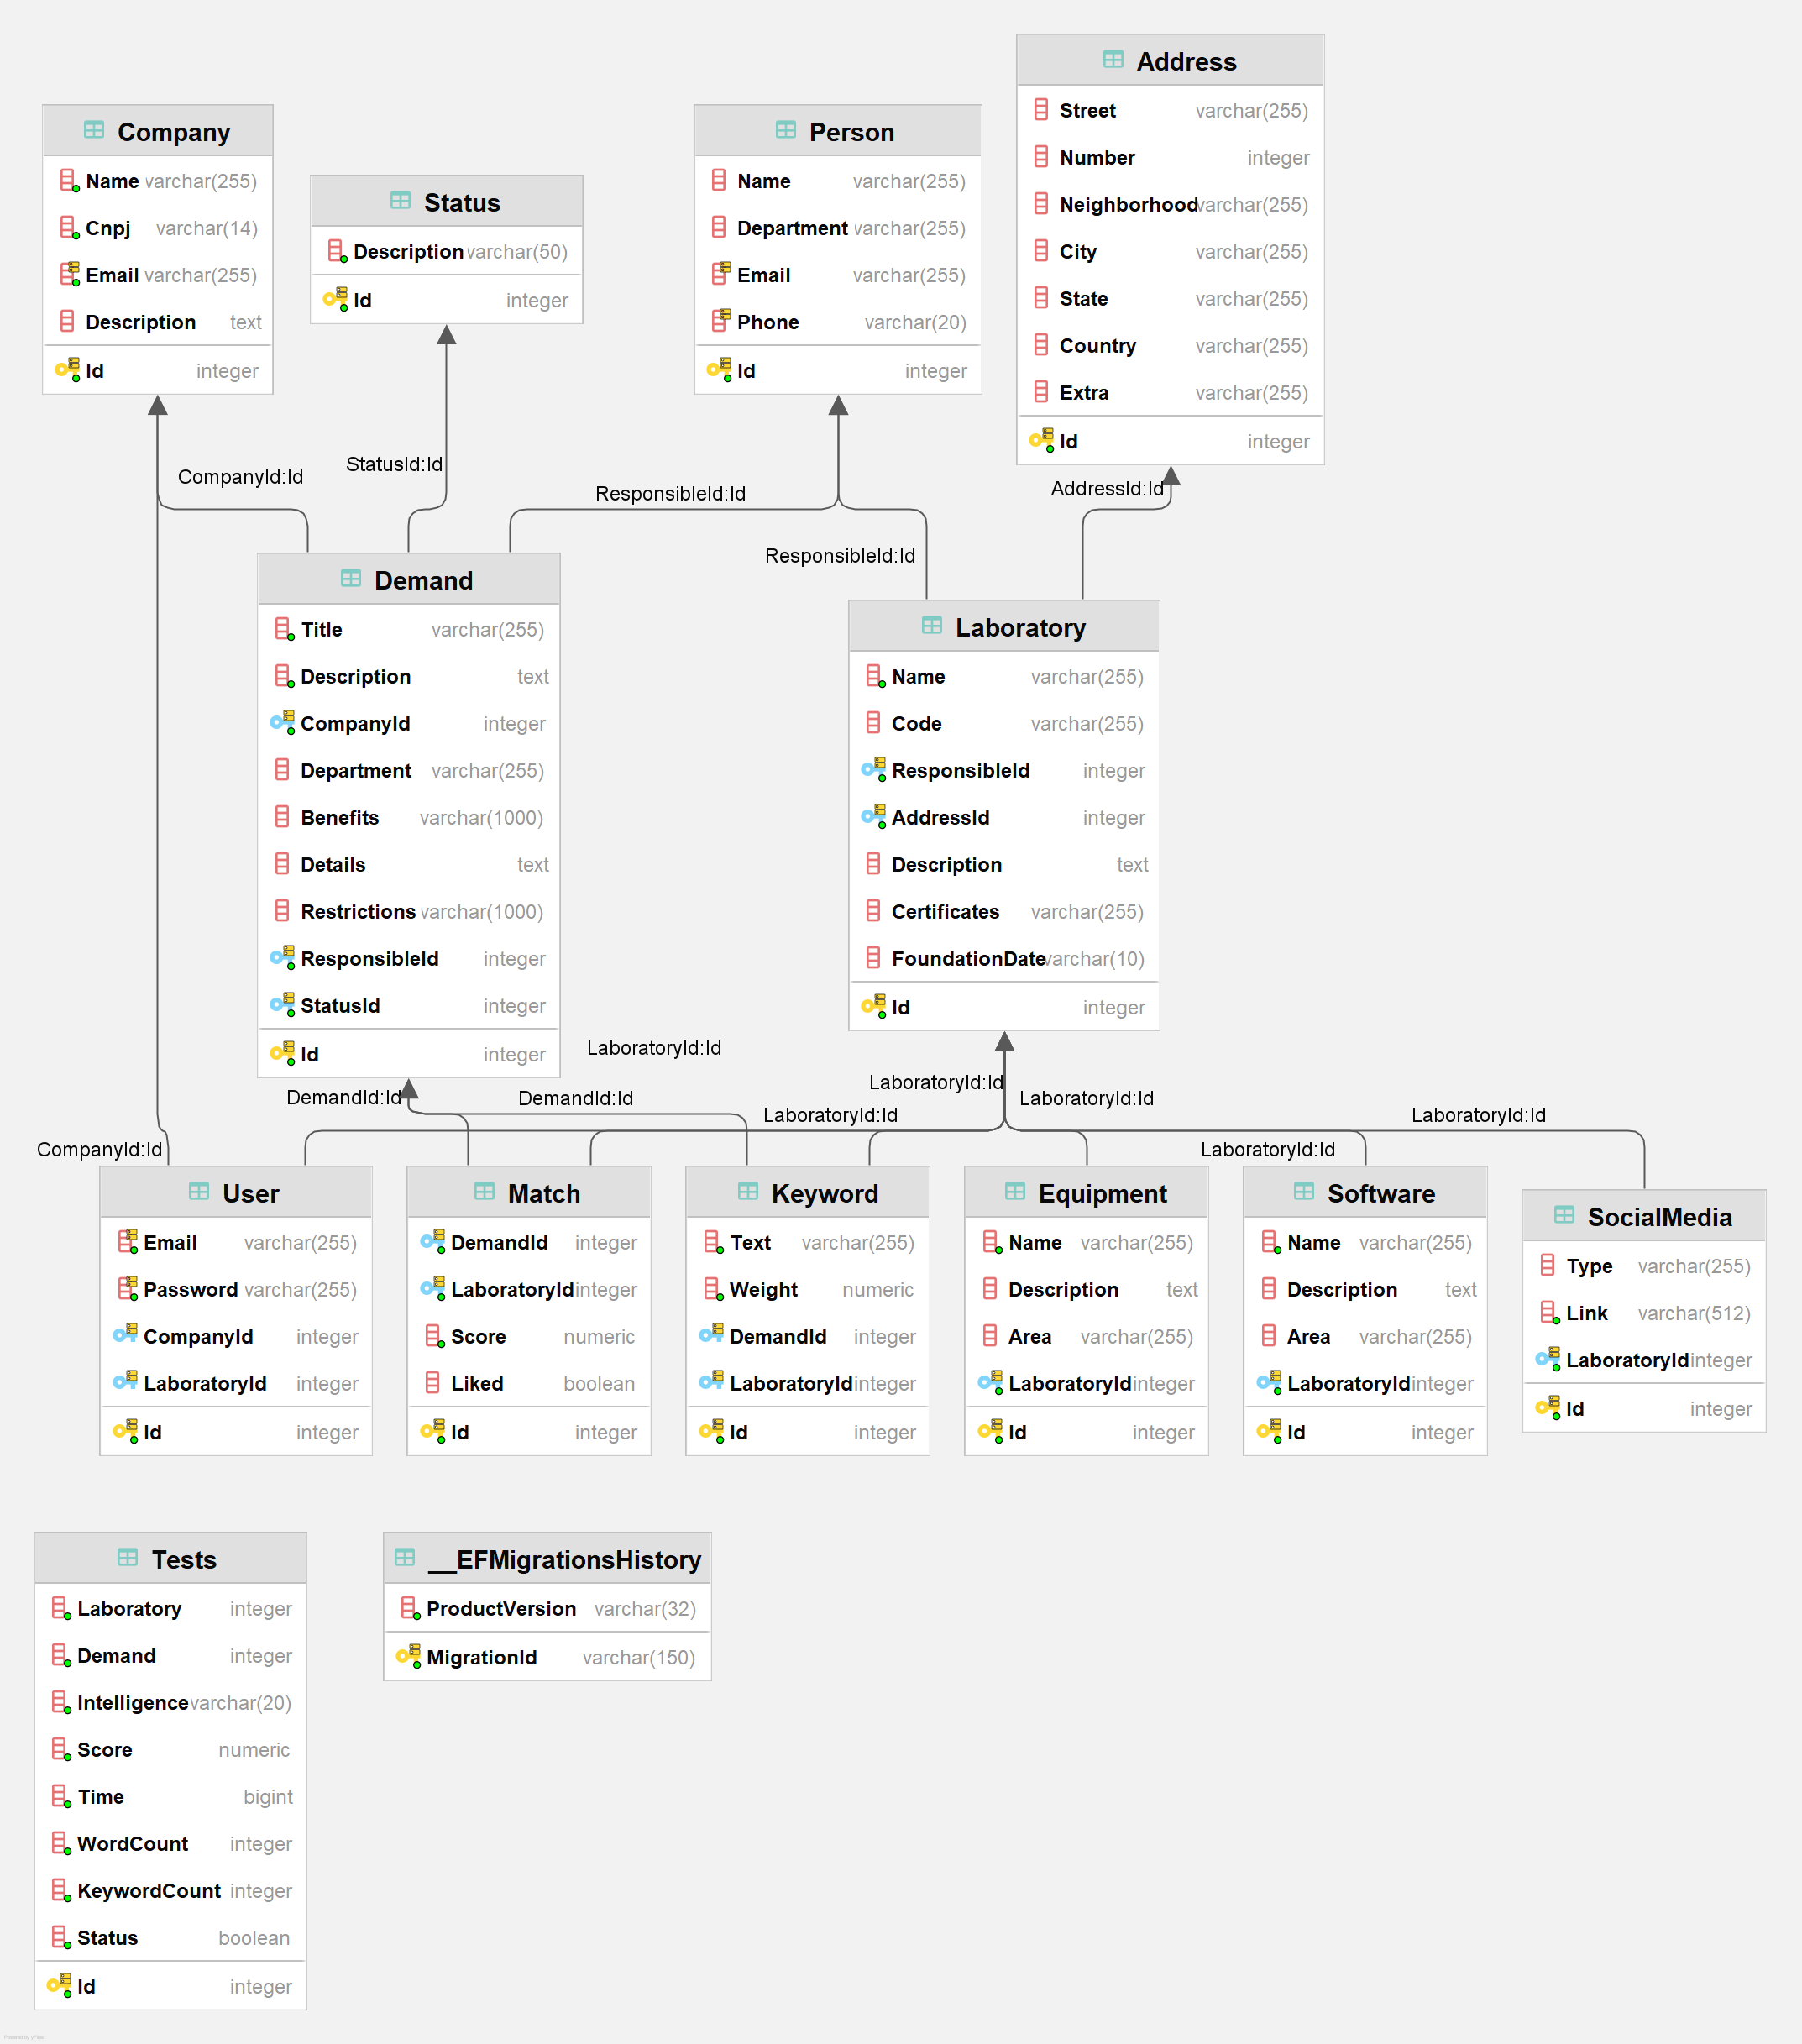
\includegraphics[scale=0.8]{ERD}
    \fonte{}
\end{figure}


% --------------------------------- Apresentação do Sistema --------------------------------- %
\section{Apresentação do sistema}\label{sec:apresentacaoSistema}

O sistema possui uma tela de login inicial, onde o usuário pode preencher seu email e senha, ou fazer um signin. Antes de realizar o signin, o usuário precisa escolher se ele é um laboratório ou organização a se registrar, e então ele é direcionado para seu respectivo formulário para preencher com suas informações.
Após realizar o login e senha, o usuário será redirecionado para sua tela principal, o qual é representado a tela principal da organização na \autoref{fig:pagina-home-org}, onde é mostrada as opções que ele poderá acessar no Aplicativo, como está demonstrado na \autoref{fig:diagrama-navegacao}.

\begin{figure}[htpb]
    \captionsetup{width=0.43\textwidth}
    \caption{Tela inicial de um usuário do tipo organização do aplicativo.}
    \label{fig:pagina-home-org}
    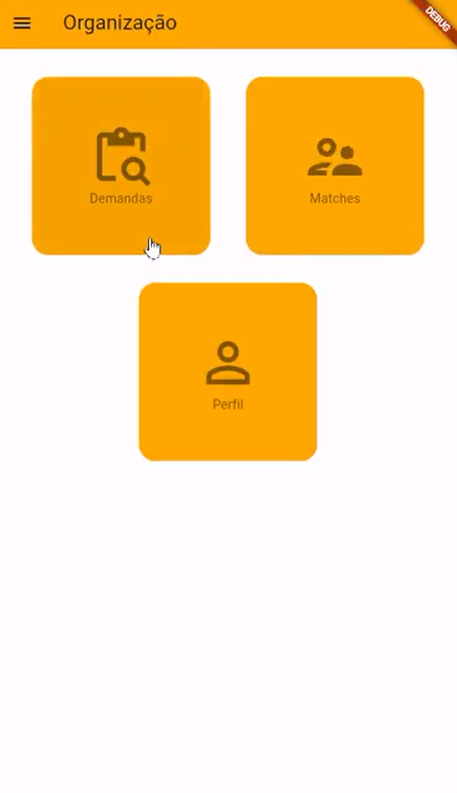
\includegraphics[scale=0.8]{pagina-home-org}
    \fonte{}
\end{figure}

\begin{figure}[htpb]
    \captionsetup{width=0.43\textwidth}
    \caption{Diagrama de navegação ao realizar o login.}
    \label{fig:diagrama-navegacao}
    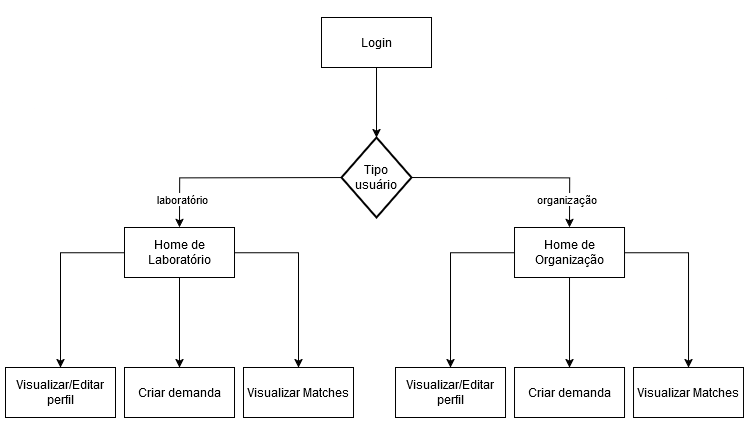
\includegraphics[scale=0.8]{diagrama-navegacao}
    \fonte{}
\end{figure}

Ou seja, uma organização poderá ver seu perfil, as demandas e os matches de todas as demandas, além dos seus detalhes, demonstrado pela \autoref{pagina-matches-detalhes} , enquanto o laboratório poderar ver seu perfil e os matches com os detalhes da demanda do organizador que o marcou como favorito.

\begin{figure}[htpb]
    \captionsetup{width=0.43\textwidth}
    \caption{Tela de detalhes de um match, com o título da demanda, e os detalhes do laboratório, de um usuário do tipo organização do aplicativo.}
    \label{fig:pagina-matches-detalhes}
    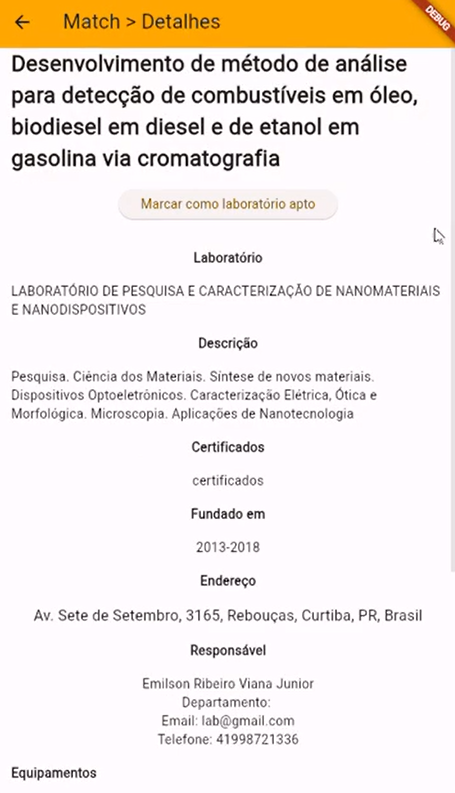
\includegraphics[scale=0.8]{pagina-matches-detalhes}
    \fonte{}
\end{figure}


% --------------------------------- Implementação do Sistema -------------------------------- %
\section{Implementação do sistema}\label{sec:implementacaoSistema}

% Nesta seção é documentada a implementação do sistema com partes relevantes ou exemplos de código, rotinas, funções. Inclui, ainda, a descrição técnica do uso de recursos (componentes, bibliotecas, etc.) da linguagem. Ressalta-se que cada orientador avaliará juntamente com seu orientado o que poderá ser descrito nesta seção. Isso sem que sejam revelados detalhes do sistema que possam comprometer seu uso comercial ou científico ou que a descrição fique muito sucinta ou superficial.

\subsection{Aplicação}\label{subsec:aplicacao}
A aplicação foi desenvolvida em Flutter, um framework, que utiliza o Dart como linguagem de programação. A interface é construída com componentes de interface para compor as páginas. Os componentes foram criados e organizados de forma independente, visando facilitar futuras implementações e alterações. Como por exemplo no \autoref{codigo:equip-form}, o componente de formulário do equipamento, que pode ser utilizado em diferentes páginas. O formulário é utilizado tanto para edição, quando para criação de equipamentos, e possui o campo "Nome" obrigatório, enquanto os campos "Descrição" e "Área" são opcionais. Quando pressionado o botão para salvar, o modal é fechado e os controllers são retornados populados para a página de lista de equipamentos, que salva os dados no banco de dados.

\begin{sourcecode}[htb]
    \caption{\label{codigo:equip-form}Classe Aluno}
    \begin{lstlisting}[frame=single, language=Dart]
class EquipmentFormPage extends StatelessWidget {
  EquipmentFormPage(
      {Key? key,
      required this.nameController,
      required this.descriptionController,
      required this.areaController})
      : super(key: key);

  ...

  @override
  Widget build(BuildContext context) {
    return Scaffold(
      body: Form(
        key: _formKey,
        child: Column(mainAxisAlignment: MainAxisAlignment.center, children: [
          const Text('Nome *'),
          Padding(
            padding: const EdgeInsets.symmetric(horizontal: 16, vertical: 16),
            child: TextFormField(
              decoration: const InputDecoration(border: OutlineInputBorder()),
              controller: nameController,
              validator: (value) {
                if (value == null || value.isEmpty) {
                  return 'Por favor, insira um nome';
                }
                return null;
              },
            ),
          ),
		  
          ...
		  
          Padding(
            padding: const EdgeInsets.symmetric(horizontal: 16, vertical: 16),
            child: ElevatedButton(
              child: const Text('Salvar'),
              onPressed: () {
                Navigator.pop(context, true);
              },
            ),
          ),

\end{lstlisting}
    \fonte{}
\end{sourcecode}

Para a comunicação com a API de Aplicação, foi utilizada o pacote nativa http, onde é possível fazer todas as requições, com todos os parâmetros necessários. Entre esses parâmetros, está o token utilizado para a autenticação da rota. O token é registrado ao realizar o login no armazenamento interno, utilizando o pacote Shared Preferences, e sendo possível buscá-lo em todas as requisições. Abaixo na \autoref{codigo:list-demands}, é possível visualizar um trecho do código utilizada para buscar as desmandas da organização logada.

\begin{sourcecode}[htb]
    \caption{\label{codigo:list-demands}Classe Aluno}
    \begin{lstlisting}[frame=single, language=Dart]
static Future<List<Demand>?> getDemand() async {
    try {
      var url = Uri.parse(
          '${ApiConstants.baseUrl}${ApiConstants.demandEndpoint}/list');
		  
	  // buscar token
      final SharedPreferences prefs = await SharedPreferences.getInstance();
      final String? token = prefs.getString('token');
	  
	  // faz requisição das demandas daquela organização
      var response =
          await http.get(url, headers: {'Authorization': 'Bearer $token'});
      if (response.statusCode == 200) {
        var body = json.decode(response.body);
		// retorna a lista de demandas
        return List<Demand>.from(body.map((item) => Demand.fromMap(item)));
      }
    } catch (e) {
	  throw Exception(e.toString());
    }
}
\end{lstlisting}
    \fonte{}
\end{sourcecode}

% Em materiais e método estão quais os recursos utilizados, neste capítulo é reportado como esses recursos foram utilizados para resolver o problema.
\subsection{API de Aplicação}\label{subsec:api-aplicacao}

\subsection{API de linguagem}\label{subsec:api-linguagens}


% Enfatizar os diferenciais do sistema: procedimentos armazenados, consultas SQL, uso de componentes, uso de padrões de projeto, a forma de uso dos recursos da linguagem. Esses diferenciais são no sentido de explicitar as vantagens, desvantagens, dificuldades e facilidades que esses recursos impetraram no desenvolvimento do sistema em termos técnicos. Esses diferenciais servirão para avaliar pela utilização ou não desses recursos, pelo menos para sistemas iguais ou semelhantes ao reportado no trabalho.

% Reportar a forma como o sistema foi verificado e validado. No sentido de verificar se os requisitos definidos para o mesmo foram atendidos. Os testes podem ser realizados pelo professor orientador, pelos professores que compõem a banca, por pessoas que serviram de base para as informações para o sistema e etc. Os testes podem ser realizados com base em um plano de testes elaborado juntamente com a análise e projeto do sistema. Para validar a implementação podem ser desenvolvidas rotinas de teste unitário.

Por falta de disponibilidade de um equipamento com sistema operacional macOS, o aplicativo foi desenvolvido apenas para a plataforma Android. Atualmente, ele conta com um arquivo instalador que precisa ser transferido para o celular para permitir a instalação direta no dispositivo. No futuro, se faz necessário disponibilizá-lo na Google Play Store, a fim de simplificar o processo de instalação e oferecer maior praticidade aos usuários

